\subsection{Silicon: the magic semi-conductor}

Silicon, which has given its name to the Silicon Valley, has joined since the late 50s the club of very important physical elements. Some greedy souls would even argue it's more important than Oxygen today: you can't make people pay for oxygen but you can make them pay for things that are built out of Silicon. Today, it's not just your typical sex-toy that uses Silicon(e) \footnote{silicone or polysiloxane is a polymer made up of siloxane - silicones consist of an inorganic silicon–oxygen backbone chain (⋯−Si−O−Si−O−Si−O−⋯) with two organic groups attached to each silicon center.}, but pretty much every electrical circuit. What makes Silicon special? How does it work? And how do we use it? 

\subsubsection{Prelude: Material Conductivity}

Conduction is not difficult to understand. You can effortlessly walk through air. It's a bit more difficult to walk through water, but you can still do it if you have enough energy. Walking through a wall is merely impossible tho, except if you, like superman, are on Kryptonite. Same idea applies to materials, which are conductive, insulating or semi conductive. You need some energy to make a semi conductive material conductive, just like walking through water. Similarly, you can only manage to make a current flow through an insulator by applying an unusually high voltage. This is also why we say that insulators have infinite impedance (in practice, it just is extremely high rather than infinite) - following Ohm's law, you need an infinitely high voltage (think Voltage on Kryptonite) to have current flowing. \\

Moving on to one of the most important concepts to understand when it comes to this chapter (and transistors physics): Band Theory. This is the model that allows us today to understand what, at an atomic level, allows a certain material to conduct (or not) electricity, and the way it does so. This also allows us to understand how the conductive properties of the material evolve as a function of external factors, such as temperature or voltage for example. 

Most of the following explanations are based on the excellent video "Band Theory (semiconductors) explained" from \textit{PhysicsHigh} Youtube Channel \footnote{\url{https://www.youtube.com/watch?v=zdmEaXnB-5Q}}. \\ 

First, we should remind ourselves that the atom is made of a nucleus with positive (and neutral) charges, and electrons around it in \textit{discrete shells}. Note: if you're not already familiar with the structure of an atom, the concepts of shells etc.., I suggest to look this up and come back here when you're familiar with it.

\begin{figure}[H]
    \centering
    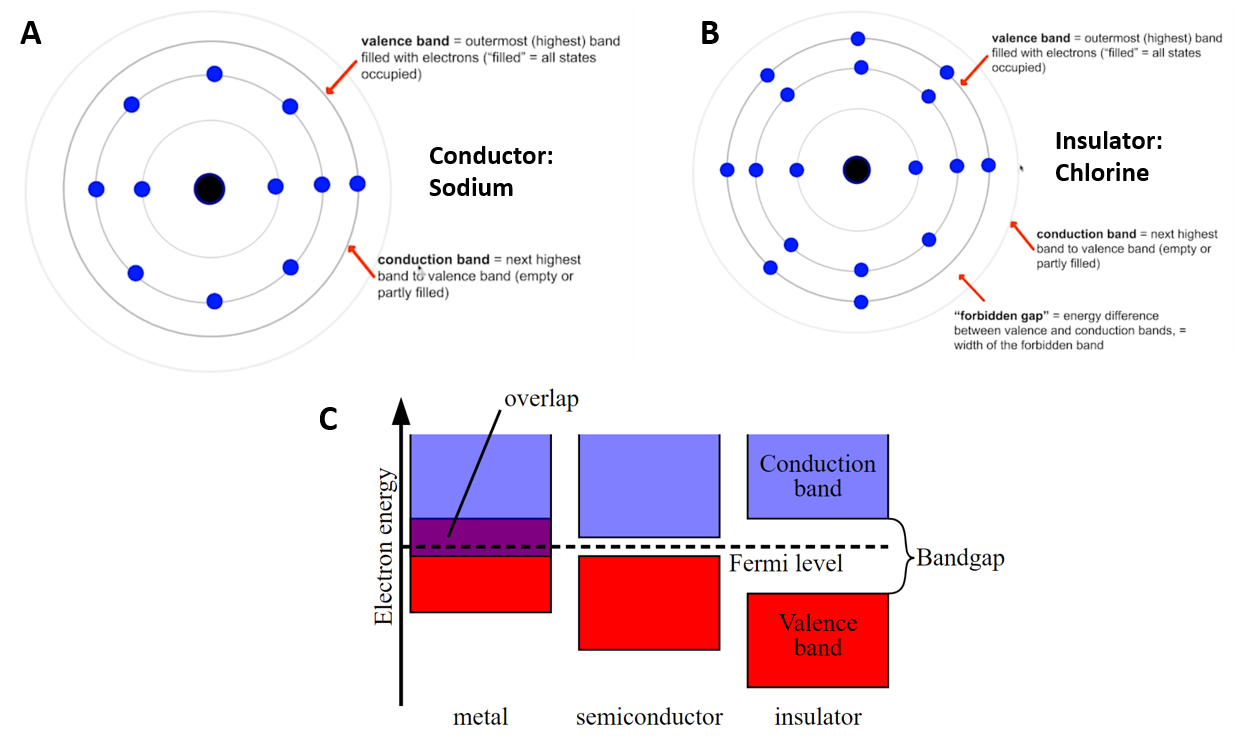
\includegraphics[width=0.95\linewidth]{../../Figures/Conduction_Energy_Band_Diagrams.PNG}
    \caption{A - Structure of Sodium Atom - a conductor. B - Structure of Chlorine Atom - an insulator. C - Simplified and generic Band Energy Diagram of conductors, semi-conductors and insulators.}
    \label{fig:Conduction}
\end{figure}

An atom such as Sodium has 11 protons and electrons, and are arranged as shown in Figure 1.A in shells - 2 in K shell, 8 in L shell and 1 in M shell.  In this specific example, the M-shell is the outermost shell, which we can also call the \textbf{valence band}. On another note, the 11th elec is alone on the valence shell (where there are 7 other spots to fill), and it thus is \textit{loosely held on that shell}, and is consequently rather free to move when a very small potential difference is applied \footnote{Understanding why this is the case requires a lot more physics, so just accept this as being true for sake of simplicity}. Sodium is thus a conductive material: it does not require much energy to have an electron moving around, which creates a current.

Now when we look at Chlorine in Figure \ref{fig:Conduction}.B, we have a different setting where the valence (outermost) shell is almost filled (7/8 electron space filled). This causes the electrons on that shell to be very tightly held together as opposed to what we saw before with Sodium. They are thus not free to move and thus cannot generate current. In order for them to move, we need to \textit{provide enough energy} for some of them to \textit{"jump" to the next shell}, where they eventually will be more free to move - the conduction band now corresponds to this next shell. To understand properly this, you need to go back to Bohr's theory that states that energy levels of electrons are quantized: it can have enough energy to reside in the M shell, and it can also have enough energy to reside in the next shell, but it cannot be in between where there exists a "forbidden gap". We therefore need to provide a very specific amount of energy for it to jump "the forbidden gap".   

You guessed it, it's basically an in-between Sodium and Chlorine that makes up for a semi-conductor. We'll look specifically at Silicon in more details soon.  

To sum things up: In a conductor, the valence band and the conduction band are overlapping: very little energy is needed to make electrons move around. In an insulator, the valence band are the conduction band are separated by a very significant energy gap: we need a huge energy supply (huge voltage for example) to make electrons in the valence band "jump" the "forbidden energy \textbf{bandgap}" to join the conduction band and finally become conductive. In a semi-conductor, we only need a very small amount of energy to have electrons make that jump, and most often, thermal energy (heat) is just enough. \\

Figure \ref{fig:Conduction}.C very simply represents the concept of what is called "Band Theory": a visual (and numerical as we'll see later) representation of energy levels of a given material. You can see that the valence band is overlapping with the conduction band in the case of a conductor, as we saw with Sodium. There is a small energy gap between the conduction band and valence band in the case of semi-conductors, and a very large energy gap in the case of insulators. Energy band diagrams therefore give you a visual representation of the amount of energy that is needed to make charges (holes and electrons as we'll see later) move from one energy state to another, and become conductive. 

\subsubsection{Thermal Consideration}

Temperature is energy, and it affects properties of materials. 

\begin{itemize}
    \item \textbf{Insulators}: at 0 K the valence band is completely filled and the conductance band is completely empty. No charge transport can take place in either bands. In room temperature, there is still a negligible amount of charge in the conduction band.
    \item \textbf{Semiconductors}: at 0 K semiconductors are equivalent to insulators. The size of the band gap $E_g$ is small in semiconductors (e.g. 1.1 eV for silicon (Si), 5 eV for diamond (C)). In semiconductors, the number of electrons available for conduction is significantly increased by thermal energy. 
    \item \textbf{Metals (conductors)}:the energy bands overlap, thus electrons and empty energy states are intermixed. At 0 K an applied electric field can generate current flow (electrons can move freely).
    \item The \textbf{Fermi Energy Level} is the difference between the highest and lowest energy of electrons at a temperature of 0 Kelvin. 
\end{itemize}

\textbf{Thermal Energy} need also be looked at. We speak of \textbf{Thermal Voltage $U_t$}: it is the mean potential caused by the thermal motion of electrons. At \textit{room temperature}, the thermal voltage is a relation between the charge $q$, Boltzmann's constant $k$ and the temperature $T$ in Kelvin: 

\begin{equation}
     U_t = \frac{kT}{q} = \frac{1.38 \cdot 10^{-23} J\cdot K^{-1} \cdot 300 K}{1.6 \cdot 10^{-19}C} \approx 25 mV = 1/40 V
\end{equation}

Note that this holds as 1 Volt = 1 Joule / 1 Coulomb.

\subsubsection{Silicon: structure, doping and properties}

\begin{figure}[H]
    \centering
    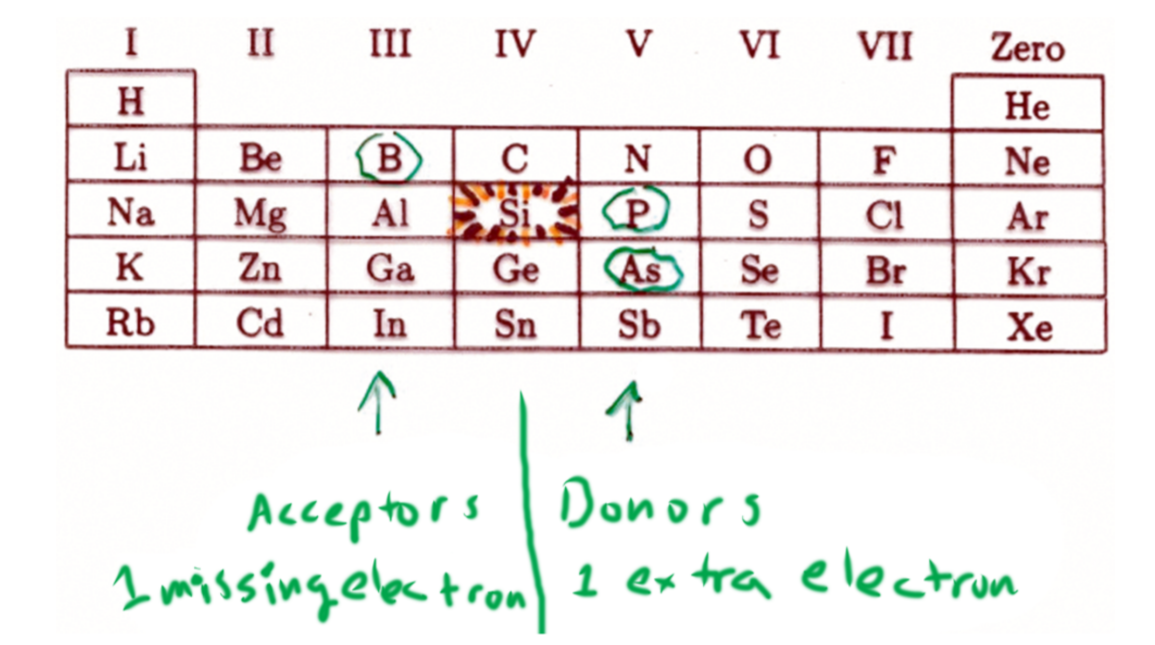
\includegraphics[width=0.95\linewidth]{../../Figures/Periodic_Table_Silicon.PNG}
    \caption{Periodic Table. Silicon and Germanium are semi-conductors. Aluminum, Boron are Acceptor Impuriy atoms: they yield free holes, Phosphorus and Arsenic are Donor Impurity Electrons: they yield free electrons. Adapted from Lecture Notes.}
    \label{fig:Periodic_Table_Conduction}
\end{figure}

This section is extensively based on Jordan Edmunds excellent lecture series on semiconductor physics \footnote{\linkhttps{https://www.youtube.com/watch?v=OVnVN0vSXn0&list=PLQms29D1RqeKGBEW8La2a7YuN5_4pSV4k}}. If you fail to understand what I write, I highly recommend checking out his explanation which go in greater depth into the topic. 

\paragraph{Silicon Structure}

\begin{figure}[H]
    \centering
    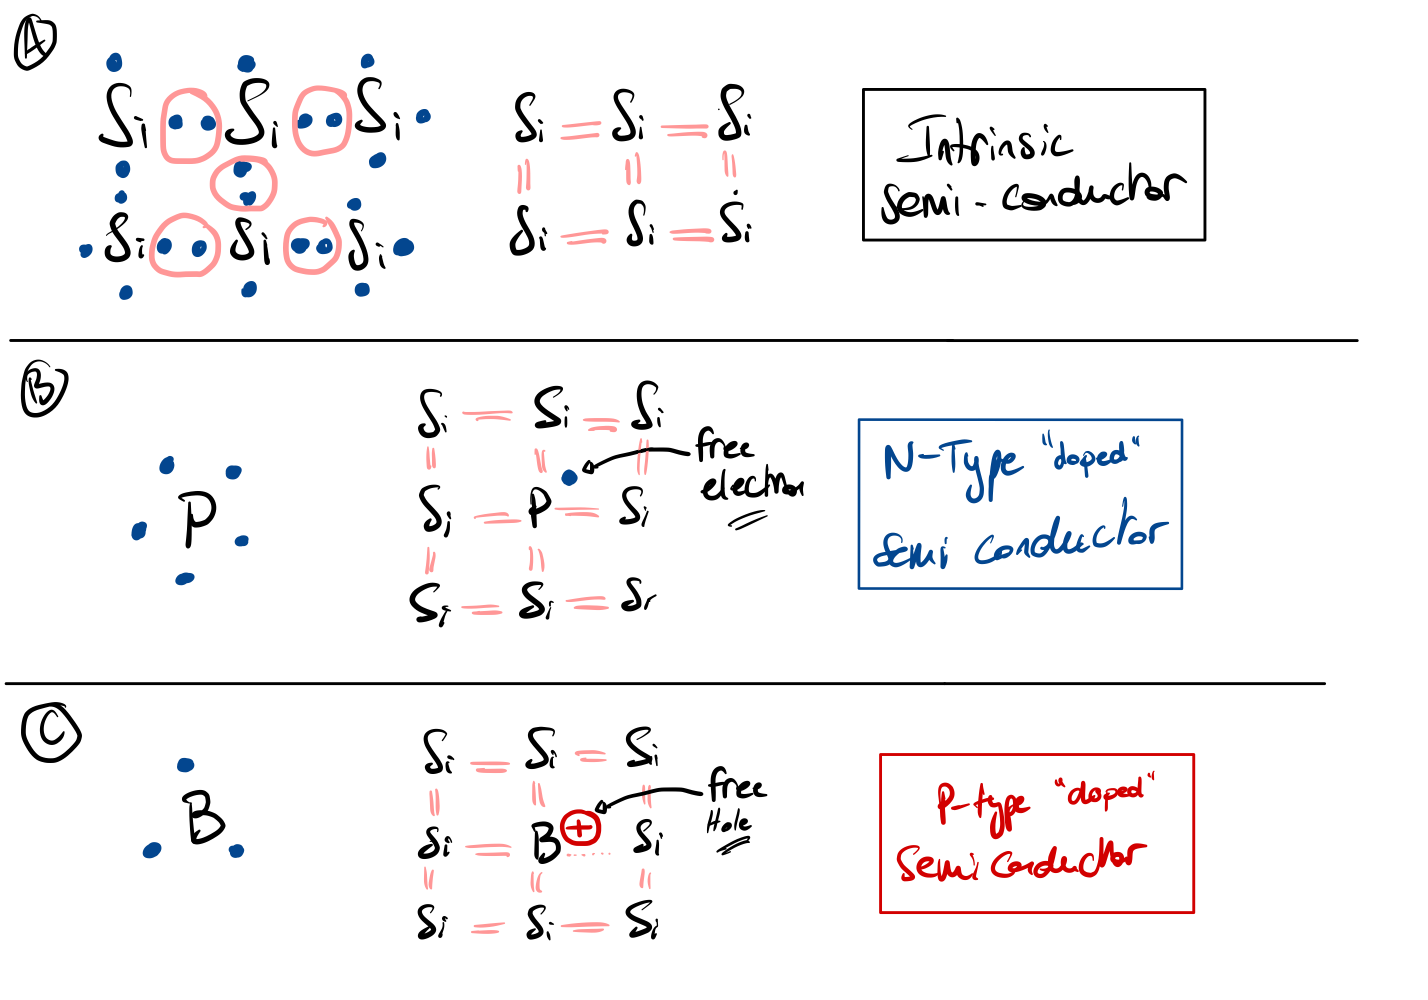
\includegraphics[width=0.85\linewidth]{../../Figures/Silicon doping.PNG}
    \caption{Intrinsic Silicon structure, and effects of doping to the structure. Blue dots are valence electrons, and red lines are "covalent bonds". Adapted from my head lol.}
    \label{fig:Silicon_Doping}
\end{figure}

Silicon is no exception to other semi conductors (and other materials) with atoms arranged in rectangular or diamond structure structures, known as \textit{crystals} *see figure \ref{fig:Silicon_Doping}.A). These structures are defined and held together by the way the valence (outermost) electrons of the atoms are distributed. Silicon's atomic number is 14: it has 14 protons and 14 electrons, including 4 in its valence (outermost) shell. It takes two neighbouring valence electrons to form a \textit{covalent bond}; this yields, in a silicon crystal, to each of the silicon atoms being bonded to 4 other silicon atoms (as shown in Figure 2.B). This is where the "diamond" analogy comes from. 
 
\paragraph{Silicon Doping}

We've just presented the structure of \textit{intrinsic} silicon (basically pure silicon). Intrinsic silicon happens to have have a high impedance at room temperature (so it conducts, but not very well conducting), this cool video \footnote{https://www.youtube.com/watch?v=k12GMjtN8aA&ab_channel=MITOpenCourseWare} reports an impedance for a ~2cm piece of Silicon of 130.000 Ohms - that's quite a high impedance . We can significantly increase the conductivity of a semiconductor by \textbf{doping it with impurities}. Doping consists in a small fraction of the semiconductor atoms in the crystal structure to be replaced by atoms of a different element, which are obviously not chosen randomly. The atoms are of course electrically neutral, and they can be of two sorts: donors and acceptors. \textbf{Donor impurity} is an atom with a valence electron \textbf{more} than the semiconductor atom, and an \textbf{acceptor impurity} is an atom with a valence electron \textbf{less} than the semiconductor atom (see Figure \ref{fig:Periodic_Table_Conduction}. Let's look at the concrete examples of Phosporus, and Boron. \\

As shown in figure \ref{fig:Silicon_Doping}.B, you can add a Phosphorus atom to silicon crystal. A Phosphorus atom has an atomic number of 15 and has 5 electrons in it's valence shell (which are the blue ones represented in the picture). It will form traditional double covalent bonds with silicon with 4 out of its 5 outermost electrons. Will now be left that extra electron which does not have anything to bond with, and is just lying there, freely moving and looking for some mate to bond with. We consider that this electron has entered the conduction band. An important thing to realize is that phosphorus has just lost one of its electrons, and it still has 15 protons. So this phosporus just turned into a phosphorus ion, and a positive one: $P^+$. The issue with that charge is that it cannot be filled by just bringing in a new electron, because that electron would not have any other electron to form a covalent bond with, which is why it lost an electron in the first place. To phrase it another way (and you'll understand in the next section why I need to phrase it another way): the positive charge accumulated in the phosphorus atom is \textbf{not} an available state which an electron can fill. As such, the positive charge in the phosphorus atom (\textit{donor impurity}) is there to stay, however the electrons are the ones moving around freely, thus justifying its name: the \textbf{N-Type Doped Silicon}. Before we move on to the next bit, note that we managed to add free electrons to crystal by doping it with phosphorus, but we actually do not change it's overall charge! It still is a neutral piece of crystal, because it has the same number of free electrons than of positively charged phosphorus ions. Pretty cool huh? \\

Now let's look at what happens when injecting a donor impurity atom: Boron (see figure \ref{fig:Silicon_Doping}.C). Boron has atomic number 5, which means that he has 3 electrons in its outermost valence shell. When injected to Silicon, it will form traditional double covalent bonds with silicon on all 3 of its valence electrons. But here is the thing, Boron still has space for more electrons on its outermost shell, it still has one available state that could potentially be filled by electrons, we say that it now carries a \textbf{hole}. A hole is not a formal charge, but it behaves just like one: it is the absence of an electron in a particular place in an atom.  So what you get is electrons hopping in this hole (and thus filling it). But when that happens, the electrons also leaves a hole behind it from the place it left. What you get is virtually a range of holes moving around freely in the \textbf{P-Type Dope Silicon} crystal.  

Now that we understood the basic idea behind doping, let's look at some band energy diagrams to see how doping affects things. 

\begin{figure}[H]
    \centering
    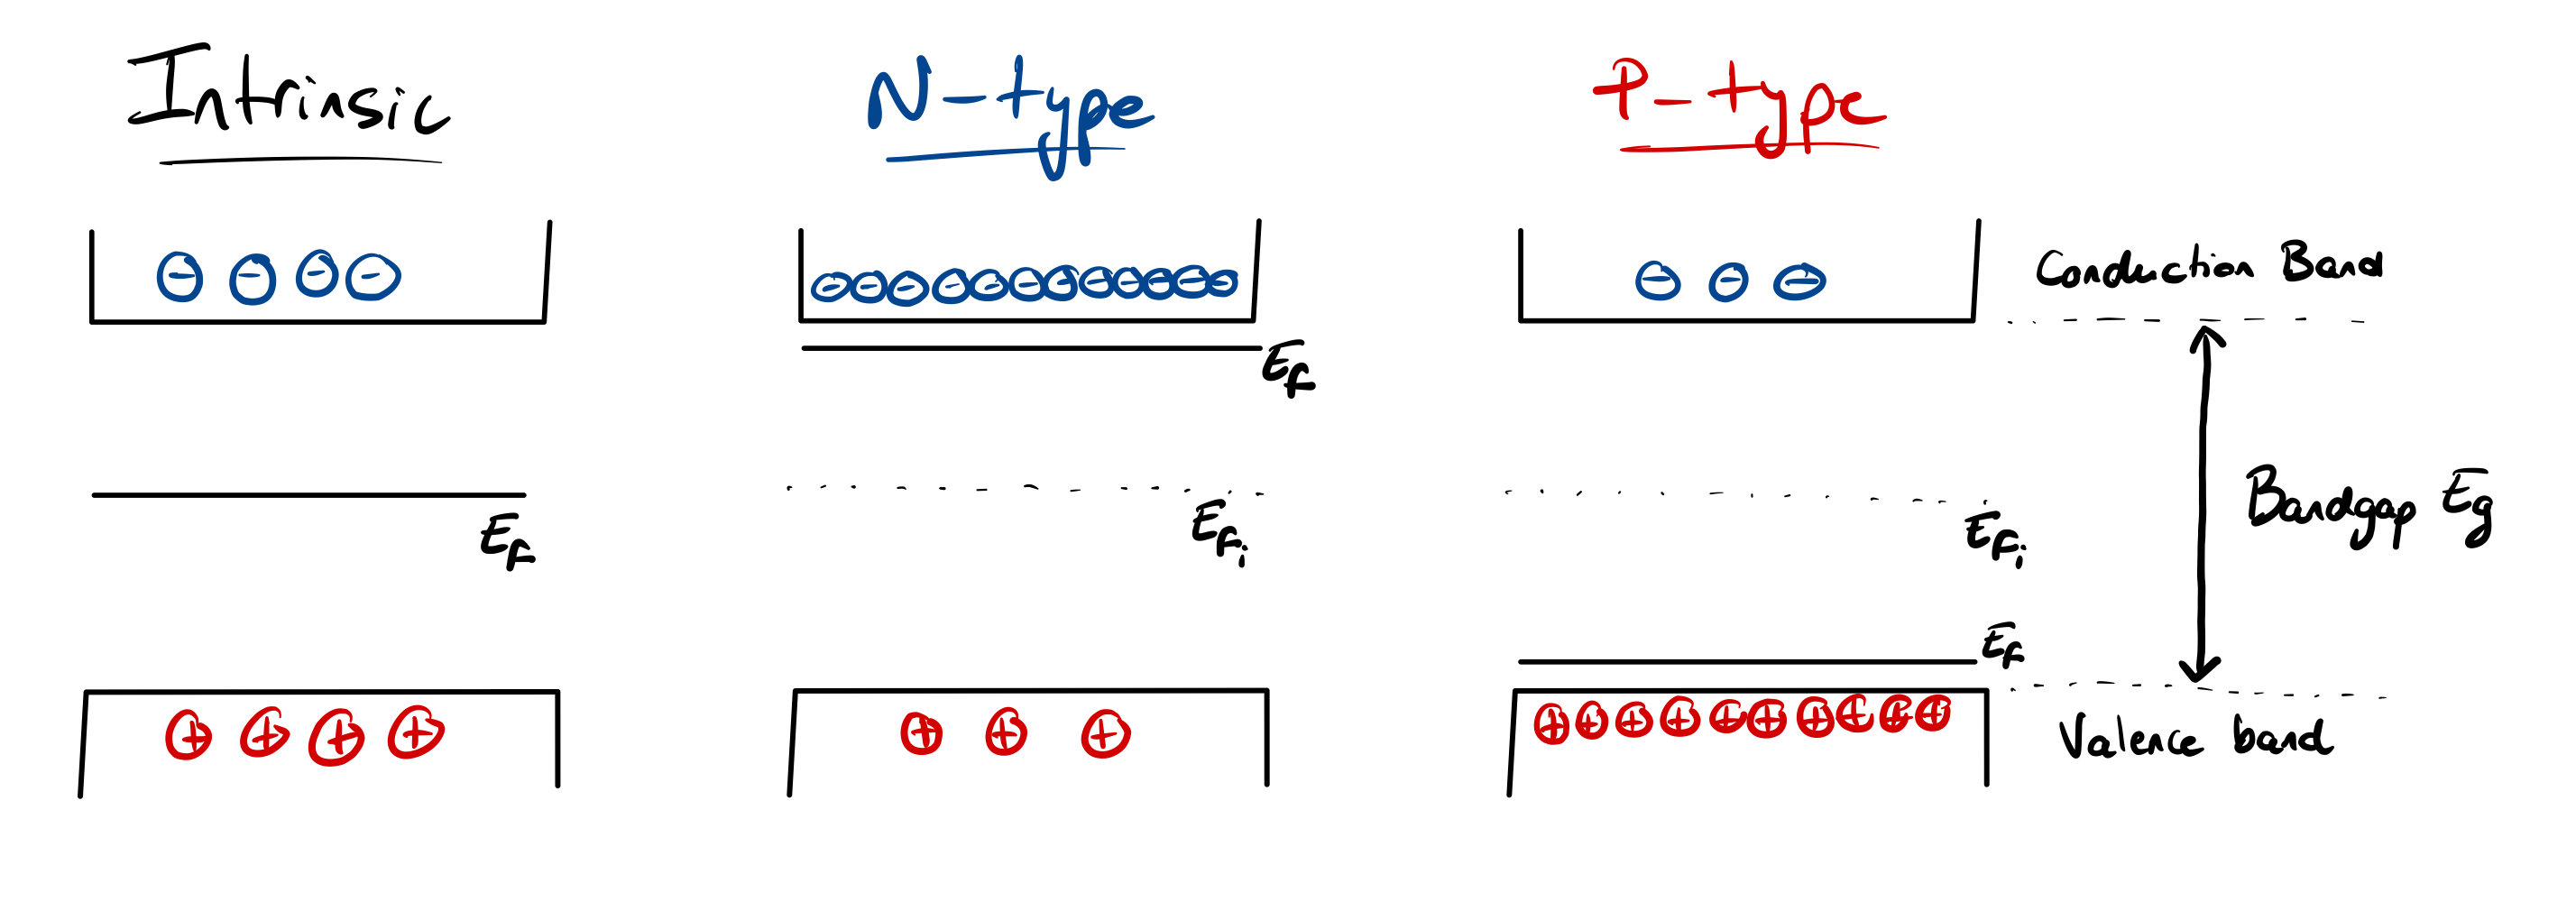
\includegraphics[width=0.95\linewidth]{../../Figures/Band diagram doping.PNG}
    \caption{Band diagram of intrinsic, N-Type and P-Type silicon. $E_{F_i}$, in dotted lines, corresponds to the intrinsic silicon Fermi Level, which is the actual Fermi Level in intrinsic graph. For P-Type and N-Type, the effective Fermi Levels are at different positions than in the intrinsic case, shown in corresponding straight lines. Adapted from a bunch of graphs I saw which didn't really make sense to me, so I drew my own. Hope it's correct lol.}
    \label{fig:Band_Diagram_Doping}
\end{figure}

To me, this is the only necessary band diagrams to understand when it comes to intrinsic vs doped semi conductors. It is necessary to understand it in order to approach properly the PN-Junction, which we will look at in the next section. In general, you should remember that the Fermi Level is determined by the doping density of charge carriers (electrons and holes). In an intrinsic semi conductor, there are (schematically) as many holes as there are free electrons, and the Fermi Level is \textit{not} in the conduction band, nor near it. Remember that the Fermi Level is the difference between the highest and lowest energy of electrons at a temperature of 0 Kelvin. That means, as we know, that an energy must be provided in order to make the material conduct electricity. When doping semi conductor in N-Type manner, we reach a level with a significantly higher level of free electrons, a lot of them already in the conduction band, thereby making the Fermi Level a lot closer to the conduction band, and thus more conductive. In the case of P-type , this is the opposite, and because the density of holes is a lot higher than the density of free electrons, the Fermi level is a lot closer to the valence band. However, one must remember that it is specifically \textit{holes in the valence band} that can move freely and generate a current flow. This is why at equivalent concentrations, N-Type and P-Type semi conductors have the same conductivity level \footnote{Take this with a grain of salt, I am really not sure whether that is the case in practice}.

Note: We can dope semiconductor to different levels. A weak P-type doping is denoted $p^-$ and a very strong N-Type doping by $n^{++}$ (you get the logic). If the semiconductor is so strongly doped that the Fermi level is within the conduction or valence band or very near the edge of one of these bands, such that a large fraction of the states at the band edge are occupied, its properties become similar to those of a metal and we speak of a
\textit{degenerate semiconductor}.

\paragraph{How is doping done in practice?}
You may wonder how does doping of silicon work in practice? The two main methods are:
\begin{itemize}
    \item Thermal diffusion: Heat silicon in closed quartz tube, pump in some vaporized phosphorus or boron, and the dopants literally diffuse into the solid silicon
    \item Ion implantation: With an electron gun type of device, release small amounts of vaporized phosphorus, arsenic or boron, accelerate the resulting ions to a high velocity and ram them into the silicon.  
\end{itemize}
At the dawn of semiconductors (from 1948 to 1960), diffusion was the primary method.